\documentclass[10pt,a4paper]{article}
\usepackage[margin=16mm]{geometry}
\usepackage[T1]{fontenc}
\usepackage[default]{sourcesanspro}
\usepackage{microtype,xcolor,tikz,tabularx,booktabs,array,fancyhdr,hyperref}
\usetikzlibrary{arrows.meta,positioning}
\definecolor{ink}{HTML}{142C40}\definecolor{teal}{HTML}{007F82}\definecolor{pale}{HTML}{EAF5F4}\definecolor{muted}{HTML}{516575}\definecolor{orange}{HTML}{C86636}
\hypersetup{colorlinks=true,urlcolor=teal,pdftitle={PRP experiments | Session processing and reference forwarding},pdfauthor={PRP experiments}}
\color{ink}\setlength{\parindent}{0pt}\setlength{\parskip}{5pt}
\pagestyle{fancy}\fancyhf{}\renewcommand{\headrulewidth}{0pt}\fancyfoot[L]{\small\color{muted}PRP EXPERIMENTS\quad /\quad EXP-001 + EXP-002\quad /\quad 17 OCT 2026}\fancyfoot[R]{\small\thepage\,/\,3}
\newcommand{\eyebrow}[1]{{\small\bfseries\color{teal}\MakeUppercase{#1}}\par}
\newcommand{\sectionlabel}[1]{\par\vspace{4pt}{\large\bfseries #1}\par}
\newcolumntype{Y}{>{\raggedright\arraybackslash}X}
\begin{document}
\eyebrow{01 / EXP-001: session processing}
\vspace{5pt}
{\fontsize{23}{26}\selectfont\bfseries Session establishment\\and per-packet processing}\par
The two experiments examine complementary prerequisites for offloading PRP processing. EXP-001 asks whether session establishment can be separated from subsequent packet processing. EXP-002 asks whether an aggregator can remove one routing layer and forward retained data without copying the body at four specific software operations. Neither experiment demonstrates a hardware accelerator.
\sectionlabel{Question and execution environment}
After an authenticated session has been established, must each received packet repeat relationship policy, handshake or key derivation? EXP-001 runs two real \textbf{libprp} endpoints with separate identities and session handles in one process. They exchange authenticated encrypted packets through in-memory byte buffers. There are no sockets, kernel modules or VMs in this experiment.
\begin{center}
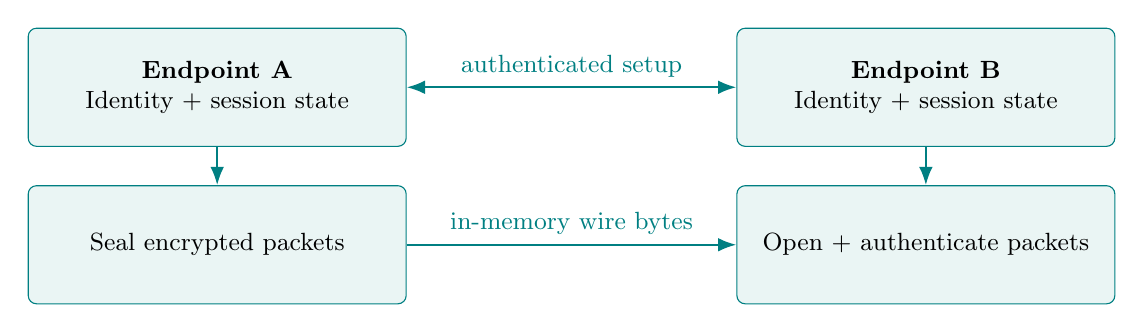
\begin{tikzpicture}[>=Latex,box/.style={draw=teal,rounded corners=3pt,fill=pale,minimum height=15mm,align=center,font=\small}]
\node[box,minimum width=48mm] (a) at(0,0) {\textbf{Endpoint A}\\Identity + session state};
\node[box,minimum width=48mm] (b) at(9,0) {\textbf{Endpoint B}\\Identity + session state};
\draw[<->,thick,teal] (a)--node[above,font=\small]{authenticated setup}(b);
\node[box,minimum width=48mm] (c) at(0,-2) {Seal encrypted packets};
\node[box,minimum width=48mm] (d) at(9,-2) {Open + authenticate packets};
\draw[->,thick,teal] (a)--(c);\draw[->,thick,teal] (b)--(d);
\draw[->,thick,teal] (c)--node[above,font=\small]{in-memory wire bytes}(d);
\end{tikzpicture}
\end{center}
\sectionlabel{What is observed}
The reproduction builds the bundled, pinned library source with native function-entry instrumentation. Observations distinguish the setup phase from the receive phase; they do not replace the library's cryptographic operations with a mock.
\begin{tabularx}{\linewidth}{@{}p{34mm}Y@{}}\toprule
\textbf{Setup work} & Relationship-policy evaluation, authenticated negotiation and session-key derivation.\\[5pt]
\textbf{Packet work} & Dispatch using installed session state, packet opening/authentication, replay protection and applicable state checks.\\\bottomrule
\end{tabularx}
\sectionlabel{Procedure and controls}
\textbf{1. Establish:} create the endpoints and complete authenticated setup.\par
\textbf{2. Exercise:} run workloads of 0, 1, 10, 1,000 and 100,000 packets, observing setup and receive separately.\par
\textbf{3. Challenge:} use deliberate regressions and lifecycle/adversarial cases to check that the observer detects forbidden repeated work and that required checks remain active.\par
\textbf{4. Verify:} validate observations and pinned inputs; print a conclusion and save the detailed evidence. Failed or incomplete runs do not establish the result.
\sectionlabel{Conclusion supported by the experiment}
In the tested sessions, packet processing reuses installed session state without repeating relationship policy, handshake or key derivation. This separation makes a bounded packet-processing path plausible for device offload. \textbf{Per-packet authentication and state validation still remain necessary.}

This is an instrumented functional experiment, not a throughput benchmark, a proof for every possible session lifecycle, or a measurement of CPU savings. Its encrypted user-space sessions are distinct from EXP-002's kernel forwarding with the NONE suite.
\vfill
\small\color{muted}Reproduction: \texttt{sudo ./run} executes both experiments and verifies their results. A successful complete cycle removes its own downloads and evidence; failures preserve diagnostics. Separate run/verify commands retain evidence for inspection. Numerical results are reported by the test, not fixed in this note.
\newpage
\normalsize\color{ink}
\eyebrow{02 / EXP-002: aggregator forwarding}
\vspace{5pt}
{\fontsize{23}{26}\selectfont\bfseries Aggregator forwarding\\and buffer reuse}\par
The experiment examines whether a PRP aggregator can remove one routing layer and prepare the outgoing packet using existing memory segments, rather than copying its complete body into another assembly buffer. CPU offload means moving work from the main CPU to a device. This test examines a prerequisite for that design, not the device itself; lower elapsed time is not required.
\sectionlabel{Topology and packet path}
\begin{center}
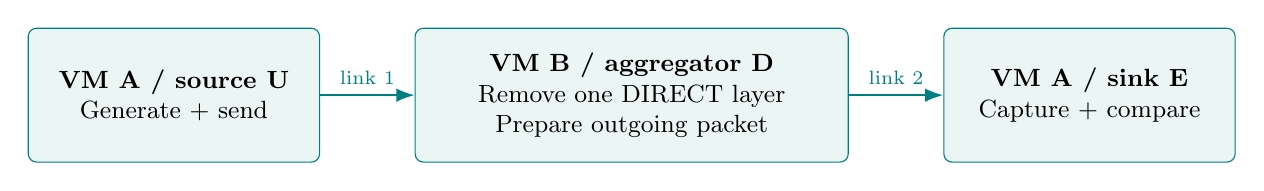
\begin{tikzpicture}[>=Latex,node distance=12mm,box/.style={draw=teal,rounded corners=3pt,fill=pale,minimum height=17mm,align=center,font=\small}]
\node[box,minimum width=37mm] (u) {\textbf{VM A / source U}\\Generate + send};
\node[box,right=of u,minimum width=55mm] (d) {\textbf{VM B / aggregator D}\\Remove one DIRECT layer\\Prepare outgoing packet};
\node[box,right=of d,minimum width=37mm] (e) {\textbf{VM A / sink E}\\Capture + compare};
\draw[->,thick,teal] (u)-- node[above,font=\scriptsize]{link 1} (d);
\draw[->,thick,teal] (d)-- node[above,font=\scriptsize]{link 2} (e);
\end{tikzpicture}
\end{center}
The source and sink are separate endpoints in VM A; the aggregator runs in VM B. Two isolated virtual Ethernet links carry the packets. Both guests use one read-only base with private disk overlays; they do not share PRP payload memory. No physical network accelerator is part of this topology.
\sectionlabel{Protocol elements used in the test}
\textbf{ONION} identifies a nested routing representation. Its outer \textbf{DIRECT} layer selects the next output and contains a child layer to forward. Removing the outer layer leaves that child intact. The aggregator does not execute the child in this hop.

The \textbf{annex} is the attached data region: in this fixture, a short prefix and a deterministic payload. The selected \textbf{NONE} session suite does not encrypt the data. Session setup remains authenticated. Annex commitments remain in the packet, but eligible transit does not recompute their hashes in the measured path. Full-byte verification is performed afterwards. NONE isolates forwarding because this lab has no cryptographic accelerator; extending the offload benefit to encrypted suites would require compatible cryptographic hardware, a hypothesis not tested here.
\sectionlabel{Reference-based forwarding}
The current profile uses one \textbf{REFERENCE} path: the aggregator prepares new framing and references retained child/annex segments. Their backing storage remains owned while it is needed. No COPY comparison is executed. References are internal memory descriptors; the actual packet bytes still travel over each virtual Ethernet link.

Four kernel counters account for logical copied bytes at \textbf{ingress, DIRECT processing, output preparation and carrier submission}. The reader takes before/after snapshots and checks their differences. Zero means those instrumented operations did not copy bytes; it does not mean the CPU made no reads or that every layer of the system is copy-free.
\sectionlabel{Procedure and interpretation}
\textbf{1. Prepare:} establish the sessions and route; generate the input and expected output independently. Payload bytes repeat 00--FF.\par
\textbf{2. Forward:} forward 32 warmup and 32 measured packets with a 1,024-byte payload. Independently capture input and output on the isolated links.\par
\textbf{3. Verify:} compare complete delivered bytes with the oracle, bind records to their context and inspect the four copy counters and retained-buffer lifecycle counters. An acknowledgement alone is insufficient.\par
\textbf{4. Interpret:} preserved delivery plus zero deltas at the four copy operations supports this reference-forwarding mechanism. It does not establish NIC offload, CPU savings or physical memory traffic. Such claims require their own measurements and hardware.
\vfill
\small\color{muted}Startup may take several minutes while both guests boot and report their kernels. Those observation times include startup and are not forwarding measurements. Delivery and copy accounting are the result; elapsed time is descriptive, not a statistical speedup claim.
\newpage
\normalsize\color{ink}
\eyebrow{03 / EXP-002: data packet layout}
\vspace{4pt}
{\fontsize{23}{26}\selectfont\bfseries PRP layer removal\\and wire representation}\par
\small Byte ranges below are inclusive, relative to the PRP unit (Ethernet payload). Multi-byte PRP integers are big-endian. $N=1024$. Kind 2 means ONION; it is \textbf{not} the session cipher-suite field.\normalsize
\begin{center}
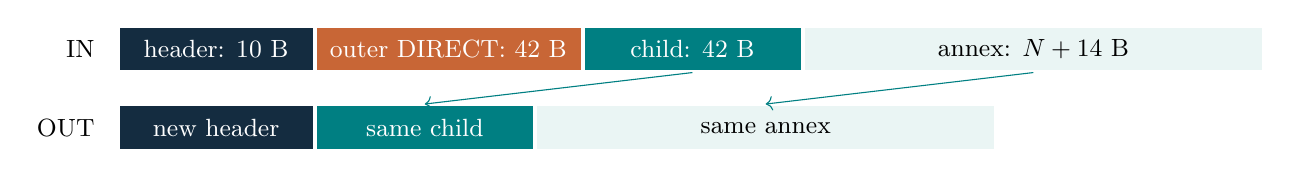
\begin{tikzpicture}[font=\small]
\node[anchor=east] at (0,0) {IN};
\fill[ink] (.2,-.27) rectangle (2.65,.27);\node[text=white] at(1.42,0){header: 10 B};
\fill[orange] (2.7,-.27) rectangle (6.05,.27);\node[text=white] at(4.37,0){outer DIRECT: 42 B};
\fill[teal] (6.1,-.27) rectangle (8.85,.27);\node[text=white] at(7.47,0){child: 42 B};
\fill[pale] (8.9,-.27) rectangle (14.7,.27);\node at(11.8,0){annex: $N+14$ B};
\node[anchor=east] at(0,-1) {OUT};
\fill[ink] (.2,-1.27) rectangle (2.65,-.73);\node[text=white] at(1.42,-1){new header};
\fill[teal] (2.7,-1.27) rectangle(5.45,-.73);\node[text=white] at(4.07,-1){same child};
\fill[pale] (5.5,-1.27) rectangle(11.3,-.73);\node at(8.4,-1){same annex};
\draw[->,teal] (7.47,-.3)--(4.07,-.7);\draw[->,teal] (11.8,-.3)--(8.4,-.7);
\end{tikzpicture}
\end{center}
\small\textbf{Diagram notation.} B means bytes; $N$ is the payload length. ``Header'' groups the 8-byte PRP record prefix and the 2-byte layer length (offsets 0--9), not the Ethernet header. The new header is also 10 bytes: the route alias and lengths change. Arrows indicate unchanged byte ranges. Block widths are schematic.\par
\renewcommand{\arraystretch}{1.12}\small
\begin{tabularx}{\linewidth}{@{}l l Y@{}}\toprule
Input offsets & Output offsets & Bytes / meaning\\\midrule
0--1 & 0--1 & 2: record count = 1\\
2--3 & 2--3 & 2: route alias 1 $\rightarrow$ 2100 (0x0834)\\
4; 5 & 4; 5 & 1 + 1: kind = 2; flags = 0\\
6--7 & 6--7 & 2: body length $N+100\rightarrow N+58$\\
8--9 & 8--9 & 2: DIRECT layer length $84\rightarrow42$\\\midrule
10--11 & removed & 2: outer commitment length = 32\\
12--43 & removed & 32: SHA256(annex), precomputed before timing\\
44--45 & removed & 2: outer branch count = 1\\
46--49 & removed & 4: egress capability = 100\\
50--51 & removed & 2: child length = 42\\\midrule
52--53 & 10--11 & 2: child commitment length = 32\\
54--85 & 12--43 & 32: child SHA256(annex), unchanged\\
86--87 & 44--45 & 2: child branch count = 1\\
88--91 & 46--49 & 4: child capability = 0xFFFFFFFF\\
92--93 & 50--51 & 2: child length = 0; aggregator does not execute this child\\\midrule
94--95; 96--97 & 52--53; 54--55 & 2 + 2: selected annex prefix fields = 17, 3\\
98--105 & 56--63 & 8: sequence = $30+i$, $i=0\ldots63$ per phase\\
106--107 & 64--65 & 2: payload length = $N$\\
108--$(N+107)$ & 66--$(N+65)$ & $N$: payload byte $j = j\bmod256$\\\bottomrule
\end{tabularx}\par
\sectionlabel{Ethernet and local submission envelopes}
\small
\textbf{Ethernet (both links).} Bytes 0--5 destination MAC; 6--11 source MAC; 12--13 EtherType \texttt{88 FB}; PRP starts at 14. MACs change between links. Captured frame lengths are $N+122$ in / $N+80$ out. Captures exclude preamble and FCS.

\textbf{Netlink submission (tested x86-64 ABI, little-endian).} 0--3 length $N+144$; 4--5 discovered family; 6--7 flags 5; 8--11 sequence; 12--15 port. 16--19: command19/version1/reserved0. 20--23: attribute length12/type23; 24--31: peer64. 32--35: attribute length$N+112$/type32; 36 onward: input PRP. \textbf{ACK36}: 0--15 Netlink header (type2); 16--19 signed error0; 20--35 original request header. An ACK alone is not delivery evidence.
\vfill
\footnotesize\color{muted}Scope: the selected single-target NONE diagnostic profile, not a general protocol specification. Signed setup/HS2 and other suites are outside this data-wire atlas. Full captured request/ACK/frame bytes and receipt digests are retained with runs outside the automatic cleanup cycle. Integrity hashes bind files; they do not independently authenticate native provenance. No claim of hardware acceleration, complete routing cost or physical zero-copy.
\end{document}
